\documentclass[10pt,a4paper]{article}
\usepackage[utf8]{inputenc}
\usepackage[italian]{babel}
\usepackage{amsmath}
\usepackage{amsfonts}
\usepackage{amssymb}
\usepackage{graphicx}
\usepackage[left=2cm,right=2cm,top=2cm,bottom=2cm]{geometry}
\newcommand{\rem}[1]{[\emph{#1}]}

\author{Gruppo BN \\ Federico Belliardo, Marco Costa, Lisa Bedini}
\title{Esperienza sull'effetto fotoelettrico}
\begin{document}

\maketitle
\section{Scopo dell'esperienza}
Obiettivo dell'esperienza � la verifica dell'effetto fotoelettrico, e di stimare la grandezza del fattore $h/e$, dove $h$ � la costante di Planck e $e$ la carica dell'elettrone\\
%forse mettere la fomrletta E = h\nu?
\section{Materiale occorrente}
\begin{itemize}
\item Lampada a LED;
\item Tubo fotomoltiplicatore Philips XP2412 B;
\item Filtri interferenziali (Balzers e Newport);
\item Scatola nera
\item Generatore di tensione continua;
\item Multimetro digitale;
\item Picoamperometro digitale;
\end{itemize}
\section{Descrizione esperimento}

Si � montato il circuito in figura \ref{fig:circuito}. Nella scatola nera erano fissati il fotomoltiplicatore e la lampada a LED che serviva da sorgente luminosa. Durante l'esperienza, si sono montati i filtri nell'apposito supporto, avendo cura che fossero ortogonali al piano di appoggio della scatola e quindi al fascio luminoso.


Per ogni filtro si � misurata la corrente in funzione del potenziale applicato ai capi del fotomoltiplicatore. Per un certo potenziale $V_0$ la corrente di elettroni (estratti per effetto fotoelettrico) che arriva all'amperometro si arresta. Questo ci consente di stimare la massima energia cinetica degli elettroni come $eV_0$, da confrontare con l'energia dei fotoni incidenti $E_{\gamma}=h\nu$.
\begin{figure}[!htb]
  \centering
  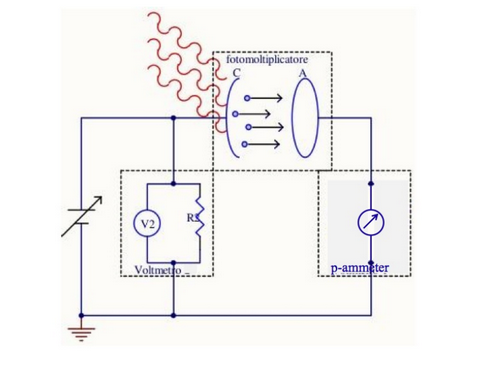
\includegraphics[scale=.5]{circuito.png}
\caption{Schema circuito dell'esperimento e di acquisizione dati.\label{circuito}}
\end{figure}


\section{Misure}

Per ogni filtro si sono prese dalle quindici alle venti misure di tensione ai capi del tubo fotomoltiplicatore e della relativa corrente.
Si � partiti da $V\simeq 0$ V e si � variato il potenziale fino a che la corrente non raggiungeva un valore asintotico. Si sono preferite prendere misure nella regione asintotica e intorno al punto in cui il grafico curvava significativamente: in questo modo ci � stato pi� facile estrarre i parametri nei fit dei punti successivi della relazione.
La tensione di frenamento � stata misurata tramite multimetro digitale. La corrente circolante nel circuito � stata misurata tramite picoamperometro.
La lettura della corrente veniva fatta dopo un tempo sufficientemente lungo da fare in modo che il valore riportato dallo strumento si fosse stabilizzato.
Come errori si sono presi gli errori strumentali riportati sui manuali dello strumento.%(0.5\% + 1 digit per il voltmetro e 0.4\% + 1 digit e 0.2\% + 1 digit per il picoamperometro, rispettivamente sulle scale dei 20 nA e dei 200 nA
Per stimare le lunghezze d'onda dei filtri, e quindi della frequenza effettiva dei fotoni incidenti, si � usata la tabella fornita (si veda la tabella \ref{tab:filtri}).
L'incertezza associata ad ogni lunghezza d'onda riportata � stata presa come la semidispersione della banda passante riportata sul data sheet per i filtri Newport, mentre per i Balzers si � assunto un valore del $2\%$ di incertezza
 \begin{table}[!ht]
\begin{center}
\begin{tabular}{|c|c|c|}
\hline 
Colore & $\lambda$ (nm) & Tipo \\ 
\hline 
Arancione & $602\pm$ & Balzers\\ 
\hline 
Giallo & $577\pm$ & Newport\\ 
\hline 
Verde & $546\pm$ & Balzers\\ 
\hline 
Verde-azzurro & $499\pm $ & Newport\\ 
\hline 
Azzurro & $ 449\pm$ & Balzers \\ 
\hline
Blu & $405\pm$ & Newport\\ 
\hline
\end{tabular} 
\caption{Caratteristiche dei filtri utilizzati \label{tab:filtri}}
\end{center}
\end{table}

Di seguito sono riportate le tabelle dei dati raccolti per ogni filtro.\\
\section{Elaborazione dati: stima potenziale di azzeramento $V_0$}
Per trovare la relazione fra frequenza dei fotoni incidenti e il relativo potenziale di azzeramento � necessario stimare dai dati quest'ultimo. Per fare ci� abbiamo usato due metodi.
\subsection{Metodo A}
Per ogni filtro si stima la corrente di emissione dall' anodo $I_A$. In prima approssimazione, si suppone che questa non dipenda significativamente dal potenziale di frenamento applicato. Pertanto si assume che la fotocorrente catodica sia $I_{C}$ sia $I-I_A$. 
Dati gli andamenti della corrente, si esegue un fit con la funzione modello $\sqrt(I_C)=aV +b$.
Una volta estratti i parametri, si trova il potenziale di azzeramento $V_0$ ponendo $I_{C}=0\rightarrow V_0=-b/a$.
Per stimare la corrente di emissione dell'anodo, si sono presi i dati in regime asintotico e si � eseguito un fit con funzione modello $y = ax +b$.
(Dati che differiscono dal valore di corrente massimo per meno del $5\%$ (valore arbitrario) vengono considerati asintotici).
Una volta ottenuto questo valore, si � eseguito un fit con la funzione modello parabolica sui dati, escludendo quelli in regime asintotico (che non possono rispettare un simile andamento).
I risultati dei fit sono riportati nelle tabelle  \ref{}
I $\chi ^2$ normalizzati sono dell'ordine delle migliaia : si vede che l'andamento non � per nulla rispettato. Inoltre i potenziali di azzeramento estratti non sono per nulla in accordo con quanto predetto dal modello, n� con quanto ottenuto nel punto successivo.
\subsection{Metodo B}
Per ogni filtro si � stimato il relativo potenziale di azzeramento $V_0$ corrispondente alla tensione per cui la corrente fotocatodica risulta compatibile con 0 entro una incertezza $\delta I$.
 Per fare ci� si � eseguito un fit per ogni set di misure con la funzione modello
\begin{equation}
I(V)=\bar{I}(e^{a(\bar{V}-V})}-1)
\end{equation}
Si osservi che con questa definizione $\bar(I)$ rappresenta il modulo della  corrente asintotica misurata.
I risultati dei fit sono riportati nella tabella \ref{tab:fitexp}.
I valori dei $\chi^2$ normalizzati sono dell'ordine delle centinaia: in effetti non ci si aspetta che l'andamento della funzione $I(V)$ sia davvero un esponenziale, ma semplicemente un andamento approssimativo con il quale estrarre dei parametri utili per i calcoli successivi.
Per ricavare $V_0$ basta risolvere l'equazione
\begin{equation}
I(V_0)=-\bar{I}+\delta(I)\Rightarrow V_0=\bar{V}+\frac{1}{a}\ln\frac{\bar{I}}{\delta I}
\end{equation} 
Dobbiamo stimare l'incertezza $\delta I$. 
Si osserva intanto che la corrente anodica non � davvero indipendente dalla differenza di potenziale applicato: guardando i dati si osserva che, anche per grandi $V$ il valore "asintotico" della corrente tende a crescere in valore assoluto.
Pertanto per stimare $\delta I$ si � preferito prendere la semidispersione dei valori delle correnti nella zona asintotica rispetto al valor medio.
Ai fini della stima non si � voluto considerare l'errore estratto dal fit del parametro $\bar{I}$: esso � irrealisticamente piccolo, persino pi� piccolo delle variazioni della corrente $I$ nel regime asintotico.
Per lo stesso motivo non si � considerato neppure l'errore strumentale (dell'ordine dello 0.4\% nelle scale usate).
Sebbene la scelta di $\delta I$ appaia abbastanza arbitraria, questa non influisce sul fit lineare finale e sul valore del coefficiente angolare della retta $h/e$: essendo sia il parametro $a$ che il valore dei $\delta I$circa lo stesso per le varie frequenze utilizzate, i vari potenziali di azzeramento $V_0$ vengono traslati della stessa quantit� se si varia $delta I$.
In tabella \ref{tab:V_0}si sono riportati i valori dei potenziali ottenuti in funzione del colore. Gli errori su $V_0$ estratti sono stati calcolati propagando gli errori dei parametri che comapiono nella formula per il calcolo di $V_0$
\begin{table}[!htb]
\begin{tabular}{|c|c|c|c|}
\hline
Colore & $\delta I$ (nA) & $V_{0, min}$(mV) & $\\sigma V_0$ (mV)\\
\hline
Giallo & 0,02 \\
Verde & 0,02 \\
Verde-Azzurro & \\
Azzurro & 0,02 \\
\end{tabular}
\caption{Valori del potenziale d azzeramento in funzione del filtro e del $\delta I$ usato\label{tab:V_0}}
\end{table}
\section{Relazione frequenza-$V_0$}
Una volta ottenuti i potenziali di azzeramento per le varie frequenze, si esegue un fit secondo la funzione modello $V_0=a\nu + b$.
Secondo il modello, $a = h/e\simeq 4.1 \mbox{J}\cdot\mbox{s}$.
I risultati del fit sono riportati in figura \ref{} e in tabella \ref{}.
Il $V_0$ per il filtro arancione non � in accordo con l'andamento teorico. In effetti a questa frequenza (pi� bassa delle altre), i fotoni hanno meno energia rispetto agli altri i casi. Il materiale eccitato nel fotomoltiplicatore � costituito da due tipi di metallo,; solo uno di questi tuttavia riesce ad essere eccitato a queste energie. Pertanto il comportamento della corrente �  diverso rispetto agli altri casi.
Anche il potenziale di azzeramento per il filtro blu non � in accordo con quanto previsto, ma non si � riuscito a trovare una spiegazione di tale fenomeno. Non si � tenuto conto di questo punto per il fit della retta.
\section{Corrente anodica}
\section{Conclusioni}


\end{document}


